\documentclass[sigconf]{acmart}
\usepackage{amsmath}
\usepackage{lmodern}
\usepackage{graphicx}
\graphicspath{{./images/}}
\usepackage{caption}
\usepackage{subcaption}
\usepackage[notransparent]{svg}
\usepackage{hyperref}  % Added for hyperlink support


% Meta information
\title{Image “Outpainting” and Hole Filling: Final Report}
\subtitle{CS 5787 Deep Learning Final Project Report}

\author{Wentao Ye}
\email{wy335@cornell.edu}
\affiliation{%
  \institution{Cornell University}
  \city{New York}
  \state{New York}
  \country{USA}
}

\author{Mitchell Krieger}
\email{mak483@cornell.edu}
\affiliation{%
  \institution{Cornell University}
  \city{New York}
  \state{New York}
  \country{USA}
}

\author{Sebastian Jay}
\email{srj63@cornell.edu}
\affiliation{%
  \institution{Cornell University}
  \city{New York}
  \state{New York}
  \country{USA}
}

% Document begins
\begin{document}

\maketitle

\section*{Team Members}
Wentao Ye (wy335), Mitchell Krieger (mak483), Sebastian Jay (srj63)

\section*{Introduction}
This paper explores the relationship between image inpainting and outpainting by training a model capable of interpolating between two disparate images, blending them seamlessly into a single coherent scene. Inpainting, or image interpolation, is a computer vision task that aims to fill in missing or removed sections of an image, ensuring the completed area integrates smoothly with the existing content. Outpainting, or image extrapolation, generates extensions of an image beyond its original borders.

Drawing inspiration from both inpainting and outpainting, our objective is to generate a transitional region between two images. Traditional inpainting requires an understanding of the context and semantics surrounding the missing area to blend edges seamlessly into the original image. Outpainting, while sharing these challenges, has less context to infer from since it involves extending the image into an unknown space. Additionally, outpainting must handle long-range semantic dependencies, ensuring the generated extensions remain consistent with the original image no matter how far the extrapolation extends. Our task incorporates these challenges and introduces an added complexity: the need for the generated region to be semantically consistent with both images.

\section*{Related Work}
To address the challenges of our task, we leverage deep learning architectures capable of capturing both the semantics at the edges of each image and the relationships between regions across the two images. Historically, Convolutional Neural Networks (CNNs) have been widely used in vision tasks due to their efficiency and ability to learn spatial relationships \cite{LeCun1998, Krizhevsky2012}. However, CNNs have inherent limitations stemming from their design. Their architecture emphasizes locality, with weight sharing across the entire input, which makes them less adept at capturing long-range dependencies or relationships between non-local regions—a key requirement for complex tasks like ours.

Transformer-based architectures, particularly those employing attention mechanisms, have shown effectiveness in both inpainting and outpainting due to their capacity to model long-range dependencies. For example, \cite{Jiahui2018} demonstrated that incorporating a contextual attention layer significantly improved inpainting performance. Vision Transformers (ViTs) introduced by \cite{Dosovitskiy2020} expanded on this by applying self-attention mechanisms to computer vision tasks, enabling the modeling of global relationships in an image. Further advancements, such as Swin Transformers \cite{Liu2021}, refined the transformer architecture for vision tasks using hierarchical computation and shifted windows to improve efficiency and adaptability. These approaches, however, remain computationally expensive and require large datasets for effective training \cite{Dascoli2021}.

Yang et al. (2019) proposed a U-Net GAN architecture to perform very long outpainting of a scene in one direction. They used Skip Horizontal Connections to connect each layer of the encoder and decoder in the Unet and an LSTM-based Recurrent Transfer Network to transfer the encoded sequences to the decoder. Using this method and generating in multiple steps, they were able to demonstrate long outpainting. Lu et al. (2021) expanded on this work by combining inpainting, outpainting, and image blending to fill in a scene between two images horizontally. They introduced a similar U-Net GAN architecture to Yang et al. but also incorporated contextual attention and a Bidirectional Content Transfer module, which used LSTMs as a bottleneck to ensure spatial and semantic consistency across two images. Our work generalizes this approach by extending it to painting between two images in multiple directions.

\section*{Datasets}
We used the \textcolor{red}{\href{https://github.com/z-x-yang/NS-Outpainting}{NS-Outpainting}} dataset to train our models. It is used in the original U-Transformer paper. We also tested our trained model on additional images sourced from the internet.

\section*{Methods}

Our primary objective is to create a system that can generate a coherent transitional region between two images, effectively producing a seamless blend. The solution we propose combines insights from both inpainting and outpainting tasks. In particular, we aim to generalize the notion of completing missing image regions (inpainting) to a setting where the "hole" is defined by two non-overlapping image segments: one at the top-right corner and another at the bottom-left corner. By doing so, we effectively create a scenario where the model must understand and synthesize a large intermediate area that harmonizes with both input segments.

This section first outlines our overall framework and then discusses the detailed architecture of the generator and discriminator, our training procedure, and the loss functions used to ensure high-quality, contextually coherent image synthesis.

\subsection*{Overall Framework}

We frame our problem as learning a conditional generative model capable of taking two (possibly disparate) image patches as input and producing the missing middle region that stitches them together. While traditional inpainting models focus on filling small masked areas within a single image, we require the ability to fill a large gap that is spatially extended and semantically complex—one that must maintain coherence across potentially very different input segments.

In our approach, we rely on a Generative Adversarial Network (GAN) framework to produce plausible completions. The key intuition is that the discriminator will guide the generator to not only produce visually appealing local textures, but also maintain global consistency. We refine this idea by using a PatchGAN discriminator, which encourages detailed local realism, and a U-Net-based generator with skip connections to retain crucial spatial information.

Figure \ref{fig:general_process} shows the general high-level process of our method. Given two partial images—one cropped from the upper-right quadrant and another from the lower-left quadrant—we concatenate them along a predetermined boundary and feed the resulting partial image (with a large missing region in the center) into our generator. The generator synthesizes the missing portion, producing a final, coherent image. The discriminator then evaluates local patches of this completed image to ensure fidelity and realism.

\begin{figure}[h!]
    \centering
    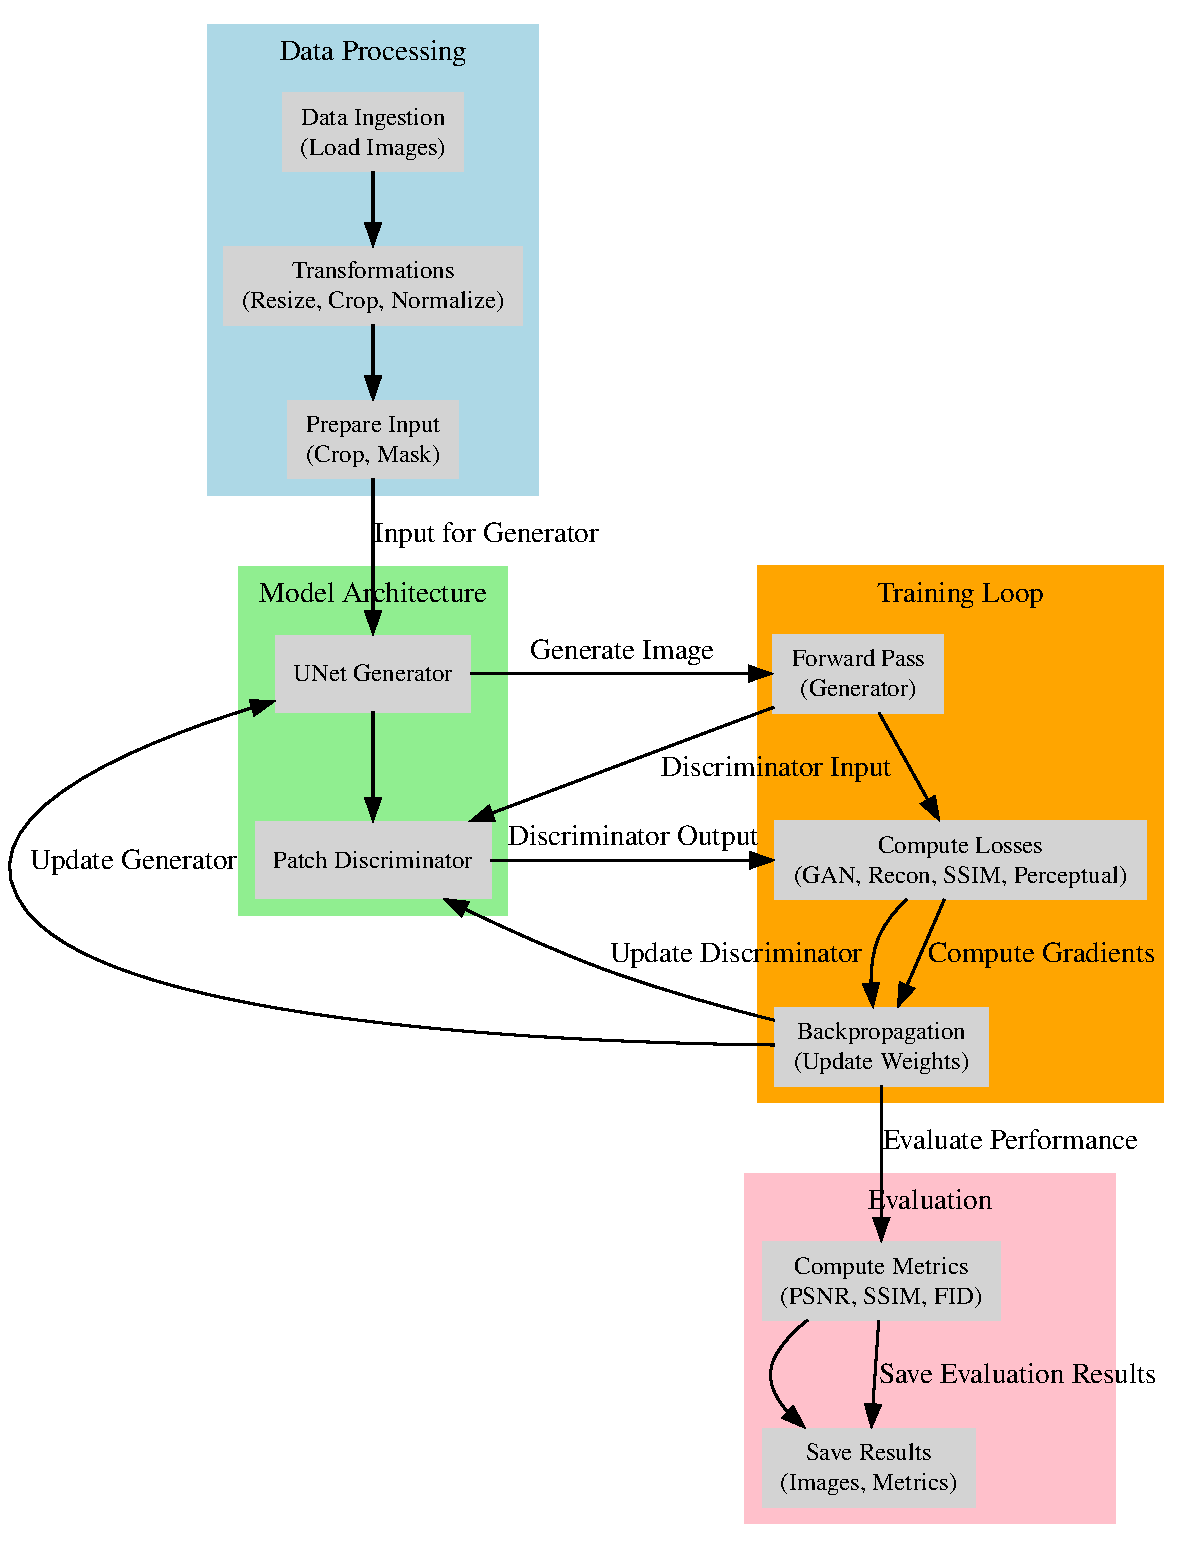
\includegraphics[width=\linewidth]{general_process.pdf}
    \caption{Overview of the general process. Two separate image patches (A and B) are combined with a large missing region in the center. Our system synthesizes a realistic, coherent image that bridges the gap between these two input patches.}
    \label{fig:general_process}
\end{figure}

\subsection*{Generator Architecture}

\noindent\textbf{U-Net-based Generator:}  
Our generator is inspired by the U-Net architecture, originally introduced for biomedical image segmentation \cite{Ronneberger2015}. The U-Net design is well-suited to our task because it uses a symmetric encoder-decoder structure with skip connections that maintain spatial details. The encoder progressively extracts increasingly abstract and semantically rich features, while the decoder gradually reconstructs the image, guided by skip connections that help preserve local structure and high-frequency details lost in downsampling.

Unlike traditional U-Nets used in segmentation, our generator must handle a complex conditional input: a partially completed scene with missing sections. We adapt the network to take in our concatenated partial images and to output a completed image of the same size. The final layer of the generator uses a Tanh activation, ensuring that output values lie in the range $[-1, 1]$ to match the normalized input image range.

Figure \ref{fig:generator} illustrates the architecture of our U-Net generator. On the left, we show the downsampling path, which encodes the input into a deep latent representation. On the right, the corresponding upsampling path decodes this latent representation back into a full-resolution image, with skip connections bridging corresponding layers.

\begin{figure}[h!]
    \centering
    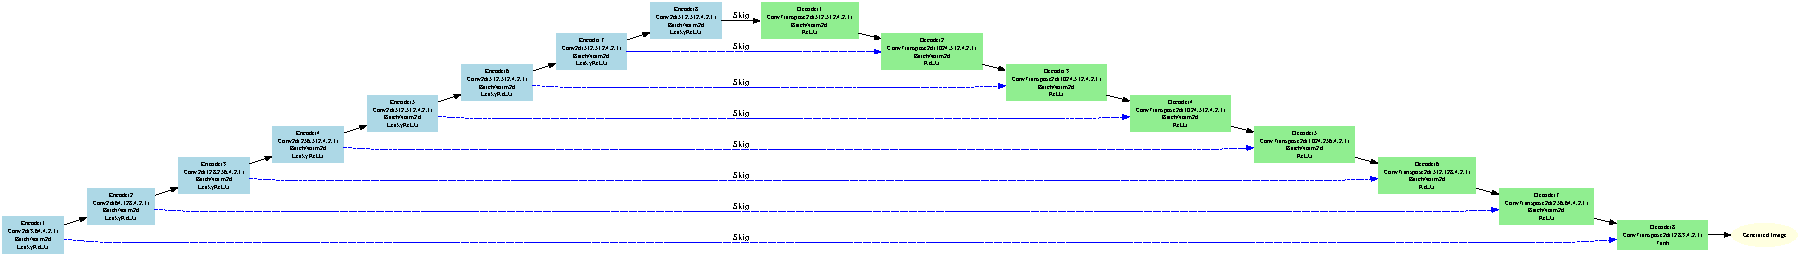
\includegraphics[width=\linewidth]{generator.pdf}
    \caption{The U-Net-based generator architecture. The input is fed into a series of convolutional layers that progressively downsample and extract features, and then the decoded representations are combined with earlier features through skip connections to produce the final completed image.}
    \label{fig:generator}
\end{figure}

\subsection*{Discriminator Architecture}

\noindent\textbf{PatchGAN Discriminator:}  
A traditional image-level discriminator that outputs a single scalar value for real/fake judgment can sometimes ignore subtle local details. To encourage the model to produce high-quality textures and local patterns, we adopt a PatchGAN discriminator \cite{Isola2017}. Instead of a single output, the PatchGAN outputs an $N \times N$ grid of values, each corresponding to the realism of a local patch in the image. This design is known to better capture local style and texture, and it prevents the generator from focusing only on global structure at the expense of local detail.

Our PatchGAN discriminator takes the generated or real completed images as input and classifies each patch as real or fake. This encourages the generator to produce realistic local details throughout the image, not just to fool a global classifier. Figure \ref{fig:discriminator} shows the schematic of our PatchGAN discriminator. It progressively downsamples the input image through convolutional layers until the spatial resolution matches that of the patch-based output. Each output value corresponds to the authenticity of a small local region of the image.

\begin{figure}[h!]
    \centering
    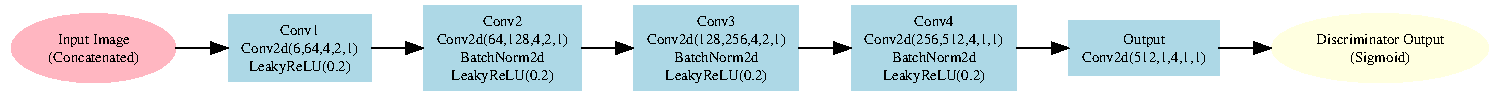
\includegraphics[width=\linewidth]{images/discriminator.pdf}
    \caption{The PatchGAN discriminator architecture. It classifies overlapping patches of the image, encouraging the generator to produce realistic local textures and details.}
    \label{fig:discriminator}
\end{figure}

\subsection*{Training Procedure}

\noindent\textbf{Adversarial Training:}  
We train our model following the adversarial learning paradigm. During training, the generator ($G$) receives two partial images and attempts to complete the missing region. The discriminator ($D$) then tries to distinguish the real, fully combined images from the synthetic outputs. We adopt a least-squares GAN (LSGAN) formulation \cite{Mao2017} for stable training. The generator’s goal is to produce samples that the discriminator classifies as real, while the discriminator aims to differentiate between real and generated samples accurately.

Our training alternates between optimizing $D$ and $G$. By iteratively improving both models, we steer the generator toward producing outputs that appear increasingly like the ground-truth combined images, balancing local detail with global coherence.

\noindent\textbf{Implementation Details:}  
We implement our model using PyTorch. The input images are normalized to $[-1, 1]$. The optimizer used is Adam \cite{Kingma2015} with a learning rate of $2 \times 10^{-4}$, $\beta_1 = 0.5$, and $\beta_2 = 0.999$. We train our models on a single GPU, and regularly monitor training by evaluating intermediate outputs to ensure visual plausibility. Model checkpoints are saved periodically.

\subsection*{Loss Functions}

\noindent\textbf{Adversarial Loss:}  
For the adversarial part, we use the least-squares objective:
\[
\mathcal{L}_{\text{GAN}} = \mathbb{E}[(D(x)-1)^2] + \mathbb{E}[D(G(x))^2],
\]
where $x$ denotes the real completed image and $G(x)$ is the generator’s output given partial input.

\noindent\textbf{Reconstruction Loss (L1 Loss):}  
To ensure that the generated regions closely approximate the ground truth, we use an L1 reconstruction loss on the masked area:
\[
\mathcal{L}_{\text{recon}} = \| x - G(x) \|_1.
\]

\noindent\textbf{Structural Similarity (SSIM) Loss:}  
Beyond pixel-level accuracy, we incorporate an SSIM loss to encourage structural fidelity:
\[
\mathcal{L}_{\text{SSIM}} = 1 - \text{SSIM}(x, G(x)),
\]
where $\text{SSIM}(\cdot,\cdot)$ measures perceptual similarity.

\noindent\textbf{Perceptual Loss:}  
We also use a perceptual loss, computed from features of a pre-trained VGG-19 network \cite{Johnson2016}, to ensure that the synthesized regions align with the high-level semantics of the original scenes:
\[
\mathcal{L}_{\text{perc}} = \sum_{l} \| \phi_l(x) - \phi_l(G(x)) \|_2,
\]
where $\phi_l(\cdot)$ is the feature map at layer $l$ of VGG-19.

\noindent\textbf{Combined Objective:}  
Our final generator objective combines these terms:
\[
\mathcal{L}_{G} = \mathcal{L}_{\text{GAN}}(G,D) + \lambda_{\text{recon}}\mathcal{L}_{\text{recon}}(G) + \lambda_{\text{SSIM}}\mathcal{L}_{\text{SSIM}}(G) + \lambda_{\text{perc}}\mathcal{L}_{\text{perc}}(G),
\]
with weights $\lambda_{\text{recon}}$, $\lambda_{\text{SSIM}}$, and $\lambda_{\text{perc}}$ controlling the importance of each component.

\subsection*{Alternative Approaches Considered}

We also considered transformer-based methods and diffusion-based inpainting models, inspired by recent work in long-range dependency modeling. However, these approaches typically require extensive computational resources and large training datasets to achieve high-quality results. For instance, Vision Transformers (ViTs) or transformer-based architectures excel at capturing global dependencies, but training them from scratch on our dataset proved challenging and computationally expensive.

Likewise, diffusion-based models are known for their high-quality samples, but training a diffusion inpainting model from scratch is computationally intensive and can struggle without massive training resources. By contrast, our proposed GAN-based approach with a U-Net generator and PatchGAN discriminator yields plausible results more efficiently, making it a practical solution within our computational constraints.

\subsection*{Justification of Approach}
Our implementation uses PyTorch, and we normalize inputs to the $[-1, 1]$ range. The models are trained using the Adam optimizer (Kingma \& Ba, 2015) with a learning rate of $2 \times 10^{-4}$ and $\beta_1 = 0.5$, $\beta_2 = 0.999$. We periodically save model checkpoints and evaluate intermediate outputs to ensure that the generator’s outputs become progressively more realistic and semantically meaningful. 

Our chosen approach strikes a balance between complexity, computational feasibility, and output quality. The U-Net generator ensures that spatial details and global coherence are preserved, while the PatchGAN discriminator encourages realistic local texture synthesis. The combination of reconstruction, SSIM, and perceptual losses helps produce both structurally consistent and perceptually convincing completions. Although state-of-the-art pretrained diffusion or transformer-based models could, in theory, produce even more photorealistic results, our method achieves a strong baseline performance with significantly fewer computational resources, making it suitable for a wide range of applications and research settings.

\section*{Experiments}

In this section, we present a comprehensive set of experiments aimed at evaluating our primary approach—a GAN-based pipeline using a U-Net generator and a PatchGAN discriminator—against two alternative diffusion-based strategies. Specifically, we compare: (1) our final GAN model, (2) a state-of-the-art pretrained Stable Diffusion model, and (3) a non-pretrained diffusion model trained from scratch. We employ both qualitative visual comparisons and quantitative metrics such as PSNR, SSIM, and FID to assess the realism, structural coherence, and overall quality of the generated images.

\subsection*{Experimental Setup}

For all experiments, we use images from the NS-Outpainting dataset. This dataset consists of wide, high-resolution panoramic images of natural scenes, which is suitable for the outpainting and image completion tasks we consider. Each image is processed by removing specific quadrants (e.g., the top-right and bottom-left portions) to create challenging input scenarios for our models. The models are then tasked with reconstructing the missing regions, effectively stitching together disparate image segments into one seamless panorama.

We report three primary experiments that correspond to different steps of complexity and difficulty in image completion:

\begin{enumerate}
    \item \textbf{Same-scene completion:} The model receives two quadrants from the \emph{same} scene as input, and must fill in the missing central region. This tests the ability to preserve global semantics and produce a consistent image with limited context.
    
    \item \textbf{Cross-scene completion:} The model receives quadrants sourced from \emph{two distinct scenes}, creating an even more challenging scenario. The model must handle semantic disparity and blend two unrelated inputs into a visually coherent transition.
    
    \item \textbf{Sparse-quadrant completion:} We increase the difficulty further by reducing the provided information, giving only partial portions of the respective quadrants (e.g., only a sub-region of the upper-right quadrant and a sub-region of the lower-left quadrant), thus creating a larger masked area in the center. This tests the robustness and generalization ability of the model under minimal input constraints.
\end{enumerate}

At each stage, we compare the outputs produced by our three modeling approaches.

\subsection*{Experiment 1: GAN-Based Model}
\label{sec:gan_exp}

Our GAN model, described in the Methods section, utilizes a U-Net-based generator and a PatchGAN discriminator. We train the model for approximately 5 hours on a single NVIDIA RTX 2070 GPU. Figure~\ref{fig:gan_step_2} shows representative results from the simpler same-scene completion scenario. Despite the challenging masked region, the GAN outputs structurally coherent images that blend smoothly across the boundaries. While not always perfect, the model preserves global context and generates plausible textures, vegetation, and lighting conditions. 

Quantitatively, as shown in Figure~\ref{fig:gan_metrics}, our GAN model achieves a PSNR and SSIM that indicate good structural integrity and perceptual quality. Although it may not achieve the absolute fidelity of more computationally expensive methods, its results are visually appealing and achieved with modest computational resources.

\begin{figure}[h!]
    \centering
    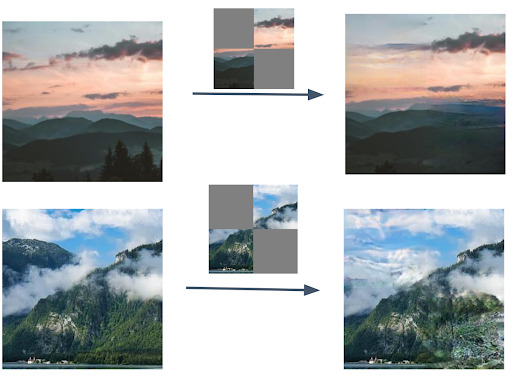
\includegraphics[width=\linewidth]{gan_step_2}
    \caption{GAN model outputs for same-scene quadrant completion. The model successfully reconstructs missing regions, preserving semantics and producing coherent textures.}
    \label{fig:gan_step_2}
\end{figure}

\begin{figure}[h!]
    \centering
    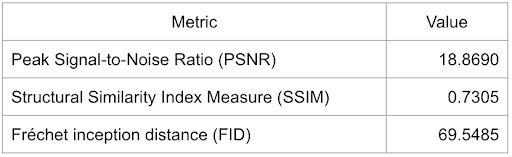
\includegraphics[width=\linewidth]{gan_metrics}
    \caption{Performance metrics of our GAN model on the test set (same-scene completion): PSNR, SSIM, and FID indicate the model’s ability to generate structurally sound and perceptually consistent outputs.}
    \label{fig:gan_metrics}
\end{figure}

Figure~\ref{fig:gan_step_4} demonstrates the GAN’s performance when blending two distinct scenes. The model still attempts to create a plausible transitional region, though subtle artifacts can appear due to stark semantic differences. Even so, it significantly outperforms random guessing and often yields a visually coherent hybrid panorama.

\begin{figure}[h!]
    \centering
    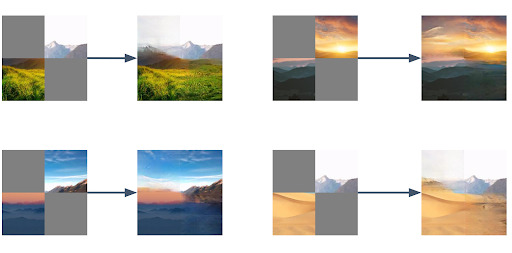
\includegraphics[width=\linewidth]{gan_step_4}
    \caption{GAN model results when attempting to blend two distinct scenes. Although the input images differ, the model generates a reasonable transitional region that attempts to merge disparate landscapes.}
    \label{fig:gan_step_4}
\end{figure}

When pushed to the sparse-quadrant scenario (Figure~\ref{fig:gan_step_6}), the model demonstrates resilience, still producing coherent completions with limited reference information. These results highlight the robust generalization capabilities of our GAN approach.

\begin{figure}[h!]
    \centering
    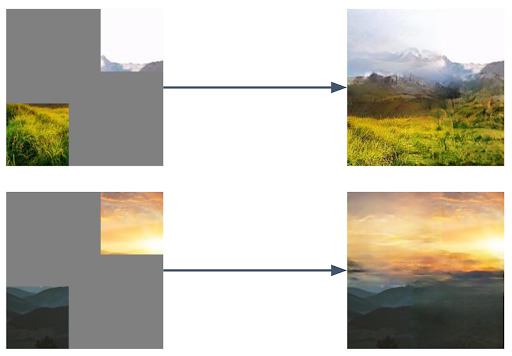
\includegraphics[width=\linewidth]{gan_step_6}
    \caption{GAN model output in the sparse-quadrant scenario, where only partial quadrant information is provided from two distinct images. The model continues to produce plausible transitions and maintain scene coherence.}
    \label{fig:gan_step_6}
\end{figure}

\subsection*{Experiment 2: Pretrained Stable Diffusion}

As a benchmark, we tested a pretrained Stable Diffusion model \cite{Rombach2022} obtained from HuggingFace. This model was extensively trained on vast image corpora using hundreds of thousands of GPU-hours, resulting in state-of-the-art generative capabilities. Figure~\ref{fig:stable_diffusion_step_2_1} and Figure~\ref{fig:stable_diffusion_step_2_2} show outputs from the same-scene completion scenario. The Stable Diffusion model’s results are often photorealistic, with high-quality textures and smooth transitions. 

When tackling the sparse-quadrant scenario, as shown in Figure~\ref{fig:stable_diffusion_step_5}, Stable Diffusion excels at creating visually convincing completions even with minimal contextual information. However, one must note the extensive compute and training resources underlying this performance—over \$600,000 in training costs \cite{Mostaque2022}—far exceeding what we used for our GAN model.

\begin{figure}[h!]
    \centering
    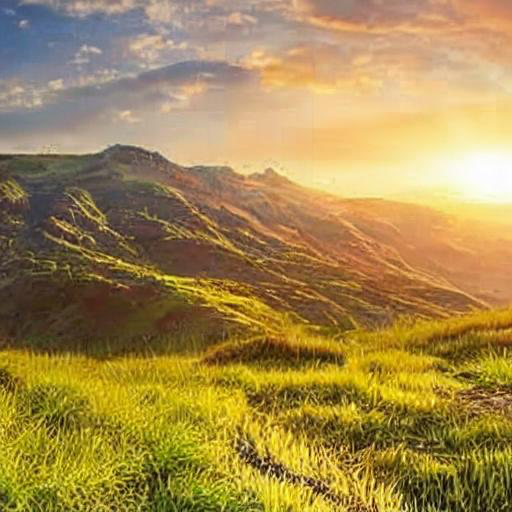
\includegraphics[width=\linewidth]{stable_diffusion_step_2_1}
    \caption{Stable Diffusion output for same-scene completion. The pretrained model produces high-quality, realistic reconstructions with rich detail and coherent lighting.}
    \label{fig:stable_diffusion_step_2_1}
\end{figure}

\begin{figure}[h!]
    \centering
    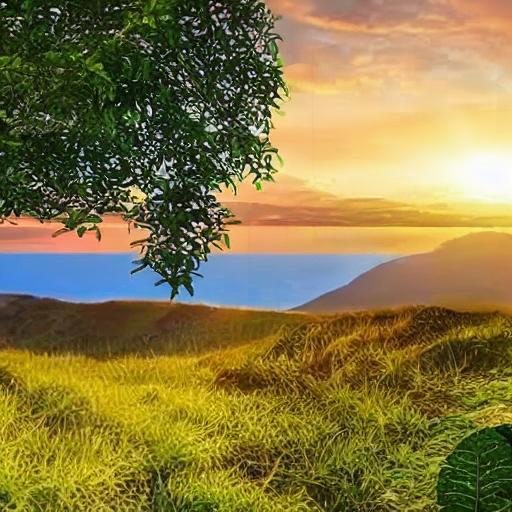
\includegraphics[width=\linewidth]{stable_diffusion_step_2_2}
    \caption{Another example of Stable Diffusion on same-scene completion. The output seamlessly integrates the missing regions with minimal artifacts.}
    \label{fig:stable_diffusion_step_2_2}
\end{figure}

\begin{figure}[h!]
    \centering
    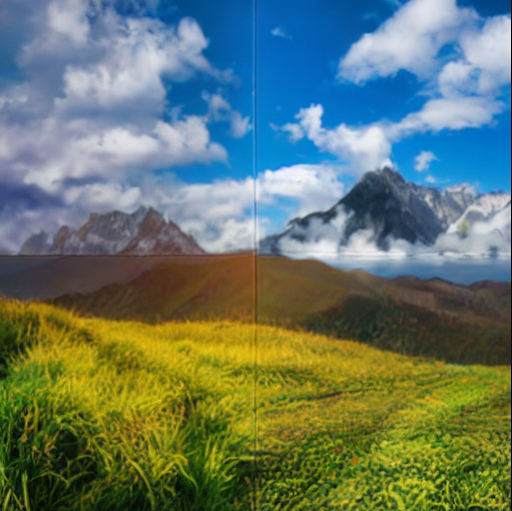
\includegraphics[width=\linewidth]{stable_diffusion_step_5}
    \caption{Stable Diffusion results for the cross-scene scenario, with two distinct scenes as input. Despite severely limited context, the pretrained model generates plausible scenes, showcasing its strong generalization and realism. Notably, unlike our model, it does not generate a single cohesive scene from the two input images and instead generates two separate scenes in its outputted montage image.}
    \label{fig:stable_diffusion_step_5}
\end{figure}

\subsection*{Experiment 3: Non-Pretrained Diffusion Model}

Finally, we attempted to train a diffusion-based model from scratch using the RePaint framework \cite{Lugmayr2022}. Unlike Stable Diffusion, which benefits from massive pretraining, our scratch-trained diffusion model is limited to the NS-Outpainting dataset and a modest training budget. Figures~\ref{fig:diffusion_step_2_1} through \ref{fig:diffusion_step_2_5} show several attempts at same-scene completion. These results are significantly weaker, with the model struggling to produce coherent global structures or realistic textures. While some color patterns and vague shapes emerge, the outputs lack semantic consistency and visually pleasing features.

\begin{figure}[h!]
    \centering
    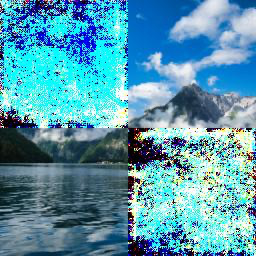
\includegraphics[width=\linewidth]{diffusion_step_2_1}
    \caption{Non-pretrained diffusion model output for same-scene completion. The generated region appears blurry and lacks coherent structure.}
    \label{fig:diffusion_step_2_1}
\end{figure}

\begin{figure}[h!]
    \centering
    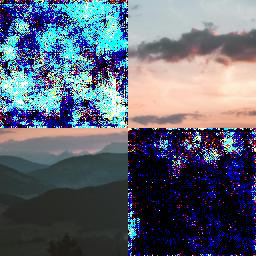
\includegraphics[width=\linewidth]{diffusion_step_2_2}
    \caption{Non-pretrained diffusion model output for same-scene completion. The model fails to reconstruct meaningful details or textures and produces amorphous shapes.}
    \label{fig:diffusion_step_2_2}
\end{figure}

\begin{figure}[h!]
    \centering
    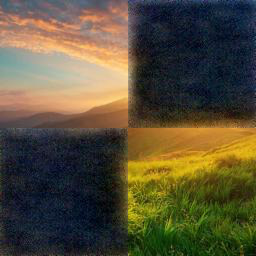
\includegraphics[width=\linewidth]{diffusion_step_2_3}
    \caption{Another example of the non-pretrained diffusion model. Although some color gradients are reasonable, no clear semantic structure emerges.}
    \label{fig:diffusion_step_2_3}
\end{figure}

\begin{figure}[h!]
    \centering
    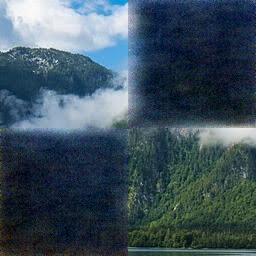
\includegraphics[width=\linewidth]{diffusion_step_2_4}
    \caption{Non-pretrained diffusion output. The image completion remains incoherent, suggesting that extensive data and compute are required for diffusion methods to match GAN-level performance.}
    \label{fig:diffusion_step_2_4}
\end{figure}

\begin{figure}[h!]
    \centering
    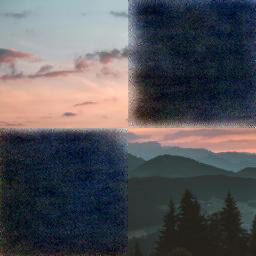
\includegraphics[width=\linewidth]{diffusion_step_2_5}
    \caption{Non-pretrained diffusion output. Attempts at structure are minimal, and the generated content does not convincingly blend with the original quadrants.}
    \label{fig:diffusion_step_2_5}
\end{figure}

\subsection*{Discussion of Results}

Comparing the three approaches:

\begin{itemize}
    \item \textbf{GAN Model:} Efficient and stable training leads to decent-quality outputs with modest computational resources. The results, especially for same-scene completion, are coherent and visually plausible. Although the GAN struggles slightly when blending very disparate scenes or with extremely sparse quadrant information, it maintains a reasonable level of realism and structural consistency.
    
    \item \textbf{Pretrained Stable Diffusion:} Achieves superior visual fidelity, realism, and detail, even in challenging scenarios. However, its success relies on massive pretraining and significantly greater computational resources. For practical scenarios without such resources, replicating Stable Diffusion’s performance from scratch is infeasible.
    
    \item \textbf{Non-Pretrained Diffusion:} Without large-scale pretraining and extensive compute, a diffusion model trained from scratch underperforms our GAN approach. The outputs are generally incoherent and lack semantic structure, highlighting the difficulty of training diffusion models in data-constrained and resource-limited settings.
\end{itemize}

Overall, our experiments show that while pretrained diffusion models can achieve remarkable realism, their resource requirements are prohibitive for many applications. In contrast, our GAN-based approach provides a strong balance between performance quality and computational feasibility, making it a practical solution for image outpainting and hole-filling tasks.

\section*{Conclusion}

As can be seen from the images above, the best results that we achieved from a model that we developed were obtained from our final GAN model, which integrates a U-Net-based generator and a PatchGAN-based discriminator.

Notably, the state of the art pretrained Stable Diffusion model \textit{“was trained using 256 Nvidia A100 GPUs on Amazon Web Services for a total of 150,000 GPU-hours, at a cost of \$600,000.”} By contrast, we achieved the results shown above with our GAN model after training it from scratch for just 5 hours on a single RTX 2070 GPU. We’d love to see what our final GAN model can achieve with a training budget of \$600,000!

\section*{Appendix}

All of our code can be found in \textcolor{red}{\href{https://github.com/yewentao256/CS5787-Final}{our repository}} on Github.

\begin{thebibliography}{9}
    \bibitem{Dascoli2021} Stéphane d’Ascoli et al., "ConViT: Improving Vision Transformers with Soft Convolutional Inductive Biases," \textit{CVPR 2021}, 2021.
    \bibitem{Dosovitskiy2020} A. Dosovitskiy, et al., "Discriminative Unsupervised Feature Learning with Exemplar Convolutional Neural Networks," \textit{IEEE Transactions on Pattern Analysis and Machine Intelligence}, 2020.
    \bibitem{Gao2022} Penglei Gao et al., "Generalised Image Outpainting with U-Transformer," \textit{CVPR 2022}.
    \bibitem{Isola2017} P. Isola, et al., "Image-to-Image Translation with Conditional Adversarial Networks," \textit{CVPR 2017}.
    \bibitem{Jiahui2018} J. Yang, et al., "Contextual Attention for Image Inpainting," \textit{CVPR 2018}.
    \bibitem{Krizhevsky2012} A. Krizhevsky, et al., "ImageNet Classification with Deep Convolutional Neural Networks," \textit{NIPS 2012}.
    \bibitem{LeCun1998} Y. LeCun, et al., "Gradient-Based Learning Applied to Document Recognition," \textit{Proceedings of the IEEE}.
    \bibitem{Liu2021} Z. Liu, et al., "Swin Transformer: Hierarchical Vision Transformer Using Shifted Windows," \textit{ICCV 2021}.
    \bibitem{Lu2021} Chia-Ni Liu, et al., "Bridging the Visual Gap: Wide-Range Image Blending," \textit{CVPR 2021}.
    \bibitem{Lugmayr2022} Andreas Lugmayr, et al., "RePaint: Inpainting Using Denoising Diffusion Probabilistic Models," \textit{CVPR 2022}.
    \bibitem{Mao2017} X. Mao, et al., "Least Squares Generative Adversarial Networks," \textit{ICCV 2017}.
    \bibitem{Mostaque2022} @EMostaque on Twitter, "The Stable Diffusion model was trained using 256 Nvidia A100 GPUs on Amazon Web Services for a total of 150,000 GPU-hours, at a cost of \$600,000." \textit{https://twitter.com/EMostaque/status/1509780730730734592}
    \bibitem{Rombach2022} Robin Rombach, et al., "High-Resolution Image Synthesis with Latent Diffusion Models," \textit{CVPR 2022}.
    \bibitem{Tang2024} Luming Tang, et al., "RealFill: Reference-Driven Generation for Authentic Image Completion," \textit{SIGGRAPH 2024}.
    \bibitem{Yang2019} Zongxin Yang, et al., "Very Long Natural Scenery Image Prediction by Outpainting," \textit{ICCV 2019}.
    \bibitem{Yu2018} Jiahui Yu et al., "Generative Image Inpainting with Contextual Attention," \textit{CVPR 2018}.
\end{thebibliography}

\end{document}
